\documentclass[american, oneside]{ecsgdp}
\usepackage[utf8]{inputenc}

% packages
\usepackage[capitalise]{cleveref} % auto format cross-references
\usepackage{svg} % SVG file compatibility

% \PassOptionsToPackage{
%         natbib=true,
%         style=apa,
%         hyperref=true,
%         backend=biber,
%         maxbibnames=99,
%         firstinits=true,
%         maxcitenames=2,
%         parentracker=true
%             }   {biblatex}
% % \usepackage{biblatex}
% \usepackage[style=apa, backend=biber]{biblatex} % for citing
% \usepackage{natbib}
%% ----------------------------------------------------------------
% Bibliography
% \usepackage{natbib}           % Use Natbib (Harvard) style for the refs
%% ----------------------------------------------------------------
% Bibliography
% \usepackage{natbib}           % Use Natbib (Harvard) style for the refs
\usepackage{babel} % dependency of BibLaTeX
\usepackage{csquotes} % dependency of BibLaTeX
\PassOptionsToPackage{
        natbib=true,
        style=authoryear-comp,
        hyperref=true,
        backend=biber,
        maxbibnames=99,
        giveninits=true,
        uniquename=init,
        maxcitenames=2,
        parentracker=true,
        url=false,
        doi=false,
        isbn=false,
        eprint=false,
        backref=false,
            }   {biblatex}
\usepackage{biblatex}
\DeclareNameAlias{sortname}{family-given} 

% remove "in:" from articles. Thanks to Herbert.
\renewbibmacro{in:}{}%
  %\ifentrytype{article}{}{%
  %\printtext{\bibstring{in}\intitlepunct}}}
 
% \renewbibmacro{in:}{%
%   \ifentrytype{inproceedings}{}{%
%   \printtext{\bibstring{in}\intitlepunct}}}

% mit "month" and "language" from Bibliography
\AtEveryBibitem{%
  \clearfield{month}{}%
  \clearlist{language}{}%
  \clearlist{location}{}%
  \clearname{editor}{}%
  \ifentrytype{inproceedings}{%
    \clearlist{publisher}%
  }
  \ifentrytype{incollection}{%
    \clearlist{publisher}%
  }
  
  }

% some natbib backwards compatibility 
\let\citealp\cite
\let\cite\textcite

% increase vertical space between bibliography items.
\setlength\bibitemsep{0.5ex}
\setlength\bibnamesep{1.2ex}

% Comma before and after journal volume. Thanks to lockstep.
\renewbibmacro*{volume+number+eid}{%
  \setunit*{\addcomma\space}% NEW
  \printfield{volume}%
  \printfield{number}%
  \printfield{eid}}
  \DeclareFieldFormat[article]{number}{(#1)}% number of a journal

% Citation Hyperlinks (not just years), thanks to Audrey.
\makeatletter
\renewbibmacro*{cite}{% Based on cite bib macro from authoryear-comp.cbx
  \iffieldundef{shorthand}
    {\ifthenelse{\ifnameundef{labelname}\OR\iffieldundef{labelyear}}
       {\printtext[bibhyperref]{% Include labelname in hyperlink
          \DeclareFieldAlias{bibhyperref}{default}% Prevent nested hyperlinks
          \usebibmacro{cite:label}%
          \setunit{\addspace}%
          \usebibmacro{cite:labeldate+extradate}}%
          \usebibmacro{cite:reinit}}
       {\iffieldequals{namehash}{\cbx@lasthash}
          {\ifthenelse{\iffieldequals{labelyear}{\cbx@lastyear}\AND
                       \(\value{multicitecount}=0\OR\iffieldundef{postnote}\)}
             {\setunit{\addcomma}%
              \usebibmacro{cite:extrayear}}
             {\setunit{\compcitedelim}%
              \usebibmacro{cite:labeldate+extradate}%
              \savefield{labelyear}{\cbx@lastyear}}}
          {\printtext[bibhyperref]{% Include labelname in hyperlink
             \DeclareFieldAlias{bibhyperref}{default}% Prevent nested hyperlinks
             \printnames{labelname}%
             \setunit{\nameyeardelim}%
             \usebibmacro{cite:labeldate+extradate}}%
             \savefield{namehash}{\cbx@lasthash}%
             \savefield{labelyear}{\cbx@lastyear}}}}
    {\usebibmacro{cite:shorthand}%
     \usebibmacro{cite:reinit}}%
  \setunit{\multicitedelim}}

\renewbibmacro*{textcite}{% Based on textcite bib macro from authoryear-comp.cbx
  \iffieldequals{namehash}{\cbx@lasthash}
    {\iffieldundef{shorthand}
       {\ifthenelse{\iffieldequals{labelyear}{\cbx@lastyear}\AND
                    \(\value{multicitecount}=0\OR\iffieldundef{postnote}\)}
          {\setunit{\addcomma}%
           \usebibmacro{cite:extrayear}}
          {\setunit{\compcitedelim}%
           \usebibmacro{cite:labeldate+extradate}%
           \savefield{labelyear}{\cbx@lastyear}}}
       {\setunit{\compcitedelim}%
        \usebibmacro{cite:shorthand}%
        \global\undef\cbx@lastyear}}
    {\ifnameundef{labelname}
       {\printtext[bibhyperref]{% Include labelname in hyperlink
          \DeclareFieldAlias{bibhyperref}{default}% Prevent nested hyperlinks
          \iffieldundef{shorthand}
            {\usebibmacro{cite:label}%
             \setunit{%
               \global\booltrue{cbx:parens}%
               \addspace\bibopenparen}%
             \ifnumequal{\value{citecount}}{1}
               {\usebibmacro{prenote}}
               {}%
             \usebibmacro{cite:labeldate+extradate}}
            {\usebibmacro{cite:shorthand}}%
          \ifthenelse{\iffieldundef{postnote}\AND
                      \(\value{multicitetotal}=0\AND\value{citetotal}=1\)}
            {\bibcloseparen% Include closing parenthesis in hyperlink
             \global\boolfalse{cbx:parens}}
            {}}}
       {\printtext[bibhyperref]{% Include labelname in hyperlink
          \DeclareFieldAlias{bibhyperref}{default}% Prevent nested hyperlinks
          \printnames{labelname}%
          \setunit{%
            \global\booltrue{cbx:parens}%
            \addspace\bibopenparen}%
          \ifnumequal{\value{citecount}}{1}
            {\usebibmacro{prenote}}
            {}%
          \iffieldundef{shorthand}
            {\iffieldundef{labelyear}
               {\usebibmacro{cite:label}}
               {\usebibmacro{cite:labeldate+extradate}}%
             \savefield{labelyear}{\cbx@lastyear}}
            {\usebibmacro{cite:shorthand}%
             \global\undef\cbx@lastyear}%
          \ifthenelse{\iffieldundef{postnote}\AND
                      \(\value{multicitetotal}=0\AND\value{citetotal}=1\)}
            {\bibcloseparen% Include closing parenthesis in hyperlink
             \global\boolfalse{cbx:parens}}
            {}}%
          \savefield{namehash}{\cbx@lasthash}}}%
  \setunit{%
    \ifbool{cbx:parens}
      {\bibcloseparen\global\boolfalse{cbx:parens}}
      {}%
    \multicitedelim}}

\makeatother

% Backrefs "cited" instead of "cit"
\DefineBibliographyStrings{english}{%
backrefpage={cited on p\adddot},
backrefpages={cited on pp\adddot}
}


\addbibresource{Latex/ref.bib}


\graphicspath{{img/}}

\begin{document}
\newcommand{\modelname}{MODELNAME }

\frontmatter
\title{Weakly-Supervised Aspect-Based Sentiment-Analysis}
\authors{Gonem Lau}
\addresses{\groupname\\\deptname\\\univname}
\date{\today}
\keywords{restaurant reviews, semantic web, sentiment analysis, natural language processing, machine learning, neural network, unsupervised learning}
\logo{logo_eur.eps}{1.75in}

% \include{digital-version}

\maketitle

\begin{abstract}
    to be written..
\end{abstract}

\tableofcontents

\mainmatter
%%%%%%%%%%%%%%%%%%%%%%%%%%%%%%%%%%%%%%%%%%%%%%%%%%%%%%%%%%%%%%%%
\chapter{Introduction} \label{chap:introduction}
This chapter presents the topic, motivations, and goals of this paper. \cref{sec:problem} introduces the problem of Aspect-Based Sentiment Analysis and explains the motivations of this field. Next, \cref{sec:objective} describes the objectives of the work and its novelties. Last, \cref{sec:structure} presents the structure of the remaining chapters. % List of Abbreviations?

\section{Problem Statement} \label{sec:problem}
With virtually everyone having access to the Web, it is not unthinkable that tons of texts could be written every second of everyday. With all that content being generated by users, it is not feasible to manually analyze all texts. Therefore, many methods in the field of Natural Language Processing (NLP) have been proposed to extract information from these textual data. One interesting subfield, Sentiment Analysis, is to discover and understand opinions from user-generated data \parencite{Liu2012SAOP}. For example, companies can improve their products or services after analyzing customer sentiments from reviews. Not only businesses profit from this field, customers benefit too. Customers can find products more easily that are up to their standards.

With Sentiment Analysis, one could analyze the text on different levels: document-level, sentence-level, or aspect-level \parencite{Liu2012SAOP}. The distinction exists because a review (document) or even a sentence could contain multiple sentiments addressing multiple aspects. For example, \cref{fig:example_review} considers a reviewer that had a positive sentiment towards the food while being more negative towards the interior.

\begin{figure}[htbp]
  \centering
  \includesvg{example_review.svg}
  \caption{An illustrative example of ABSA subtasks.}
  \label{fig:example_review}
\end{figure}

This paper focuses on Aspect-Based Sentiment Analysis (ABSA), which mainly aims to extract all aspects of a product or service mentioned in a review, and classify the sentiment for each aspect \parencite{Liu2012SAOP}. However, the task is not strictly defined. For example, some datasets provide the aspect category whereas others provide targets, in which targets are the explicit aspect expressions found in a sentence. Sentiment classification can also differ per dataset. For example, the SemEval datasets provided by \textcite{Pontiki2015SemEval} and \textcite{Pontiki2016SemEval} define sentiment as positive, neutral, or negative, while the Yelp 2014 dataset \parencite{Tang2016Yelp} ranks sentiment on a 5 star range.

In more detail, the target could be described with one or multiple aspect categories, and optionally with the aspect term(s), while sentiment could be described with the sentiment polarity and optionally with the opinion term(s). Therefore, ABSA research could be divided into four subtasks: Aspect Term Extraction (ATE), Aspect Category Detection (ACD), Opinion Term Extraction (OTE), and Aspect Sentiment Classification (ASC) \parencite{Zhang2022Survey}. ATE aims to extract explicit aspect expressions within a given text. ACD categorizes the aspects into a predefined set of categories. OTE extracts explicit opinion terms towards aspects. ASC predicts the sentiment polarity for each aspect within a sentence. To illustrate these tasks with the previous example in \cref{fig:example_review}, ATE extracts the explicit terms ``food'' and ``interior''. ACD categorizes the targets to \texttt{FOOD\#QUALITY} and \texttt{AMBIENCE\#GENERAL}, respectively. OTE, extracts the explicit terms ``Excellent'' and ``could use some help''. ASC predicts the aspects to be positive and negative, respectively. The main focus of this research is Aspect Category Sentiment Detection (ACSD), which contains three multi-task tasks found in ABSA: ATE, ACD, and ASC. Therefore, the OTE task will not be investigated.

\section{Research Objective} \label{sec:objective}
ABSA solutions can be classified in three different types: rule-based methods, supervised machine-learning, and unsupervised machine-learning \parencite{Schouten2016Survey}. In the beginning, rule-based approaches were investigated such as the model proposed by \textcite{Hu2004Rules}. However, with more access to computational power, machine learning and especially neural models have been growing in popularity as seen when comparing by the earliest survey by \textcite{Schouten2016Survey} and a more recent survey by \textcite{Zhang2022Survey}. Rule-based approaches felt out of favor as they required careful constructions which involve lots of manual effort. Yet, some models exploit both approaches with excellent performance \parencite{Trusca2020HAABSA++, Meskele2020ALDONAr}. Until recently, the majority of the machine-learning approaches focuses on supervised models which yield great results \parencite{Zhang2022Survey}. However, supervised approaches require large datasets which take substantial effort to construct, especially on aspect level. Therefore, un- or semi-supervised models are one of the ways that have been devised to overcome the struggles presented by previous approaches \parencite{He2017ABAE}. Unsupervised models show great potential as their performance itches closer and closer to supervised methods. %%%%%%%%%% REFERENCE %%%%%%%%

As stated above, the field of ABSA is not confined to a single task. Nevertheless, most methods address a single subtask rather than multiple. For example, the sophisticated supervised LCR-Rot-hop++ \parencite{Trusca2020HAABSA++} model exploits the position of the target. Therefore, the data would have to include the explicit aspect expression, or ATE has to be performed beforehand. Yet, some efforts have been made to create a multi-task solution by considering a set of inter-related dependencies from the four subtasks. One of which is the Aspect category and Sentiment Classification (CASC) \parencite{Kumar2021CASC} model, which is a weakly-supervised approach to the ACD and ASC tasks. CASC follows a three-step process. First, class vocabularies for aspect and sentiment categories are constructed using only seed words. Second, unlabeled data is turned into labeled data in a weakly-supervised manner. Third and last, a multi-task neural model is implemented to perform ACD and ASC.

The authors of CASC used a simple linear layer in the third step. Therefore, swapping the linear layer with a more sophisticated neural model is unexplored territory. In this paper, we explore injecting LCR-Rot-hop++ \parencite{Trusca2020HAABSA++} into CASC \parencite{Kumar2021CASC}. Furthermore, LCR-Rot-hop++ was originally constructed to only perform ASC. However, we also explore the performance of LCR-Rot-hop++ for ACD. As noted earlier, the second step of CASC is modified to also perform ATE to exploit positional information of aspects. In short, our research question can be summarized as follows:

\begin{center}
    \textit{How to exploit an sophisticated neural model in a weakly-supervised ABSA framework?}
\end{center}

As mentioned above, ABSA is a helpful tool for both businesses and customers. With the help of unsupervised models, businesses do not have to create a large division of their staff to manually go through their reviews. With unsupervised multi-task ABSA models being relatively unexplored, we propose a novel model which we compare against unsupervised models. Second, the model extends the first model to exploit the positional information of the target by replacing the simple model in the three step with a modified LCR-Rot-hop++ model. Comparisons are made using the SemEval dataset challenges \parencite{Pontiki2015SemEval, Pontiki2016SemEval}. In short, our main contributions can be summarized as follows:

\begin{itemize}
    \item We extend CASC by extracting aspect terms during the second step. That implies the model is able to perform the ATE task indirectly besides the ACD and ASC tasks.
    \item We adapt and compare the CASC model in step three. The linear layer gets replaced by the sophisticated LCR-Rot-hop++ model. Therefore, positional information gets exploited unlike in the simple linear layer.
    \item We explore the performance effects of LCR-Rot-hop++ for the ACD task. The model is originally performed for ASC only. Therefore, inter-dependent information between ACD and ASC are exploited by employing multi-task learning.
\end{itemize}

The implementation is based on code provided by \textcite{Kumar2021CASC}. It uses both the PyTorch and TensorFlow frameworks. Both frameworks are very popular amongst researchers and businesses for implementing their neural network models. The source code for this paper can be found at \url{https://github.com/Gogonemnem/BSc2-thesis-ba-qm}.

\section{Thesis Structure} \label{sec:structure}
The paper continues as follows. \cref{chap:related_work} provides an overview of prior approaches proposed in ABSA. Next, \cref{chap:data} illustrates the datasets used in the empirical analysis. Afterwards, the proposed models in this paper are thoroughly explained in \cref{chap:methodology}. In \cref{chap:results}, the performance of the proposed models is compared against other state-of-the-art approaches. Last, main findings are presented in \cref{chap:remarks} together with some limitations and suggestions for future research.

%%%%%%%%%%%%%%%%%%%%%%%%%%%%%%%%%%%%%%%%%%%%%%%%%%%%%%%%%%%%%%%%
\chapter{Related Work} \label{chap:related_work}
This chapter presents an overview and a review of previous works. First, \cref{sec:paradigms} explains the different paradigms that are often used to solve the ABSA task. Furthermore, it dives into why some paradigms are more amenable to unsupervised learning. Next, \cref{sec:single} explores methods that have been proposed in recent years to solve subtasks in ABSA individually. Afterwards, \cref{sec:multi-task} shows recent progress towards solving multiple subtasks using multi-task learning 

\section{Model Paradigms} \label{sec:paradigms}
Before describing the works appearing in ABSA, we briefly explore four common modeling paradigms adopted from NLP: Sequence-level Classification (SeqClass), Token-level Classification (TokenClass), Machine Reading Comprehension (MRC), and Sequence-to-Sequence modeling (Seq2Seq).

%!!!!!!!! This paragraph needs a bit more explanation
In SeqClass, input text is usually encoded to extract task-specific features which get used by a classifier to predict the correct label. Next, TokenClass is also known as sequence labeling or sequence tagging, which assigns a label to each token in the input text. In contrast to SeqClass, TokenClass classifies every token within a sequence rather than the sequence itself. For ABSA, it is common to use the BIOES tagging scheme (B-beginning, I-inside, O-outside, E-ending, and S-singleton). Then, MRC extracts spans of texts from input text conditionally on a given query. For example, a query could be ``What are the aspect terms?'' which then extracts the start and end position of the text spans corresponding to the aspects. Therefore, MRC does not have to extract the inner tokens unlike TokenClass. Last, Seq2Seq aims to generate an output sequence from an input sequence. For example, this paradigm has been applied to translating texts.

Although the TokenClass paradigm has seen some unsupervised methods, such as in identification of idiomatic expression \parencite{Fazly2009UnsupervisedTokenClass}, ABSA has basically seen no progress for unsupervised learning using this paradigm. The same holds for the MRC and Seq2Seq paradigm. Other fields such as question and answering \parencite{Cui2020UnsupervisedMRC} and translation \parencite{Ramachandran2017UnsupervisedSeq2Seq} have seen some progress. However, ABSA has not seen progress as it is uncommon to use MRC and Seq2Seq methods for ABSA tasks \parencite{Zhang2022Survey}. Therefore, mostly unsupervised SeqClass methods are explored due to the compatibility with the ABSA tasks.

\section{Single-tasks ABSA} \label{sec:single}
This section presents different subtasks within ABSA handled as single tasks. However, the OTE task will not be discussed as we do not aim to extract opinion expressions in the multi-task model. In other words, the following paragraphs present the progress made in ATE, ACD, and ASC.

\subsection{Aspect Term Extraction} \label{sec:ATE}
With ATE aiming to extract the explicit aspect expressions, supervised methods often formulate the subtask as a TokenClass problem. The reason is that usually the aspect expression can be found in the text input.

% \todo{papers from Yin CRF, Liu RNN, Xu CNN}

While supervised approaches yield impressive results, they often require large labeled datasets. The neural models are not bottlenecked by their simplicity but rather by the available data \parencite{Huang2020JASen}, which motivates the latest trend of creating un- and semi-supervised models.  

% \todo{small examples of non-neural solutions?}

Many approaches have been explored but there is no framework that has a clear lead. \textcite{He2017ABAE} propose the Attention-based Aspect Extraction (ABAE) model which de-emphasizes irrelevant words through an attention mechanism to improve the coherence of extracted aspects. \textcite{Liao2019LCC+GBC} propose LCC+GBC, which leverages local and global contexts to extract aspects. Then, \textcite{Tulkens2020CAt} propose CAt, a simple solution in which they only use a Part of Speech (POS) tagger and domain-specific word embeddings to extract aspects using a contrastive attention mechanism. The authors mention that a potential drawback of this method might be its simplicity. Although the model performs well, it might perform worse on more difficult or sophisticated dataset challenges. 
%\todo{mention Shi's paper contrastive framework? I might not employ any contrastive mechanisms}


\subsection{Aspect Category Detection} \label{sec:ACD}
With ACD aiming to identify the categories of a sentence or aspect, the SeqClass paradigm is usually applied. One advantage of applying ACD over ATE is that no explicit aspect expressions have to be in the sentence. For example, ``It's expensive and gross'' could be categorized to the \texttt{PRICE} and \texttt{FOOD} categories, whereas ATE can not identify what is being reviewed. Furthermore, ACD predicts the categories jointly, whereas ATE extracts aspects separately, thus losing information. Therefore, supervised methods approach the task as a multi-label assignment problem. 

However, tackling ACD in an unsupervised manner has a different approach. Therefore, supervised methods are not discussed. Unsupervised ACD loses the advantages over ATE mentioned in the previous paragraph. The approaches often consist of ATE and, subsequently, single-label ACD on the aspect terms. In other words, sentences without targets can't be categorized. First, candidate aspect terms, which are likely to be the aspects, are extracted. Then, those candidate terms are mapped or clustered to the pre-defined aspect categories. One of the earlier unsupervised ACD methods was ABAE mentioned in the previous section. One drawback of this model is that the learned aspects need to be mapped manually. Therefore, \textcite{Karamanolakis2019Seed} propose a teacher-student framework that extends the ABAE model by leveraging seed words eliminating the need to manually assigning the learned aspects. % If Shi included, also include here.

\subsection{Aspect Sentiment Classification} \label{sec:ASC}
Similar to ACD, ASC is usually implemented with the SeqClass paradigm, labeling each aspect to a polarity score. Although ASC has seen many supervised methods through the years \parencite{Zhang2022Survey}, the single task of ASC has not seen much progress in the field of unsupervised learning. The most likely reason is that input data about aspects are needed to classify sentiment on an aspect level. Input data can be provided in two different ways, as the aspect term or category. Differences are subtle, but one interesting difference is that positional information can be exploited with aspect term data.

An interesting framework that exploits such positioning is the LCR-Rot model by \textcite{Zheng2018LCR-Rot} which splits sentences in a left context, target, and right context. This model has been extended to exploit ontology reasoning, multiple attention mechanisms and contextual embeddings \parencite{Schouten2017Ontology, Wallaart2019HAABSA, Trusca2020HAABSA++}.

\section{Multi-task ABSA} \label{sec:multi-task}

Models for multi-task learning has seen many variants. This is also because some authors focus on different combinations of different tasks. 

Early studies in unsupervised learning that jointly extract aspect and sentiments are mostly based on Latent Lirichlet Allocation (LDA) \parencite{Blei2003LDA}. \textcite{Xu2012JAS} propose the Joint Aspect/Sentiment model (JAS) which adapts LDA by introducing sentiment-related variables and integrating sentiment prior knowledge. \textcite{Zhao2010MaxEnt-LDA} further extract aspect-specific opinions in a generative process. \textcite{Wang2015Boltzmann} introduced a Restricted Boltzmann Machine-based (RBM) approach to extract aspect and sentiment by treating them as hidden variables in RBM.

Recent studies propose weakly-supervised methods for the compound task.
\textcite{Zhuang2020JASA} introduce Joint Aspect-Sentiment Analysis (JASA) which extends the ABAE model to learn aspect/sentiment representations. Furthermore, they make use of multi-task learning by letting the aspect and sentiment representations interact. Therefore, aspect-specific opinion (such as delicious for food) are learned. \textcite{Huang2020JASen} propose the Joint Aspect Sentiment (JASen) model. First, the model learns joint topic embeddings while encouraging topic distinctiveness. Then, neural layers pre- and self-train by embedding-based predictions which generalize the word-level discriminative information on unlabeled data. 

Most recently, \textcite{Kumar2021CASC} propose a different method. The Context-aware Aspect and Sentiment Classification (CASC) model turns unlabeled data into noisy labeled data. After that, neural models are trained on said labeled data. The process of turning unlabeled data to labeled data is only weakly-supervised and requires a small amount of seed words per aspect/sentiment category, which turns into a full-fledged vocabulary list. 

%%%%%%%%%%%%%%%%%%%%%%%%%%%%%%%%%%%%%%%%%%%%%%%%%%%%%%%%%%%%%%%%
\chapter{Data} \label{chap:data}
This chapter presents the data used for this research. \cref{sec:evaluation_data} presents the dataset used for evaluating the model and comparing to other approaches. Furthermore, additional pre-processing steps are explained. Then, \cref{sec:training_data} presents the dataset which is used for training the neural model.

\section{Evaluation dataset} \label{sec:evaluation_data}
The datasets used for validation the are the SemEval 2015 and SemEval 2016 datasets \parencite{Pontiki2015SemEval, Pontiki2016SemEval}. Specifically, our analysis focuses on restaurant reviews. Each review consists of one or more sentences, and each sentence contains the sentiment on one or more aspects. The sentiment can either be positive, neutral, or negative. In our research we focus evaluating on explicit aspects, which means that the aspect is present in the sentence. 
LATER VERSIONS INCLUDE A TABLE WITH STATISTICS %!!!!!!!! Show data.... How many removed
Figure \ref{fig:example_semeval} shows an example sentence from the SemEval 2016 dataset in the XML markup language. This example further illustrates that sentences may contain multiple aspects with different sentiment polarities.
% Table \ref{describeData} gives the descriptive statistics of the SemEval 2015 and the SemEval 2016 data sets. One can notice that there are relatively few neutral reviews. Furthermore, in most data the positive class is the majority class, except for the test data of the SemEval 2015 data set. 
The SemEval 2016 dataset contains the SemEval 2015 dataset and is considerably larger. 

\begin{table}[htbp]
\centering
\caption{Descriptive statistics of the Yelp, SemEval 2015 and SemEval 2016 datasets.}
\label{tab:data}
\resizebox{\textwidth}{!}{%
\begin{tabular}{@{\extracolsep{4pt}}llllllllllll@{}}
\hline
Dataset                            & \multicolumn{2}{c}{Positive} & \multicolumn{2}{c}{Negative} & \multicolumn{2}{c}{Food} & \multicolumn{2}{c}{Place} & \multicolumn{2}{c}{Service} & Total \\ \cline{2-3} \cline{4-5} \cline{6-7} \cline{8-9} \cline{10-11} \cline{12-12}  
                                   & Freq.         & \%           & Freq.         & \%           & Freq.       & \%         & Freq.        & \%         & Freq.         & \%          & Freq. \\ \hline
Yelp CASC                          & 1543          & 69\%         & 706           & 31\%         & 881         & 39\%       & 781          & 35\%       & 587           & 26\%        & 2249  \\
Yelp Max                           & 1744          & 74\%         & 601           & 26\%         & 689         & 29\%       & 920          & 39\%       & 736           & 31\%        & 2345  \\
SemEval 2015                       & 82            & 46\%         & 96            & 54\%         & 83          & 47\%       & 55           & 31\%       & 40            & 22\%        & 178   \\
SemEval 2016                       & 159           & 78\%         & 46            & 22\%         & 88          & 43\%       & 73           & 36\%       & 44            & 21\%        & 205   \\
SemEval 2015 Single label   - Gold & 127           & 59\%         & 90            & 41\%         & 106         & 49\%       & 66           & 30\%       & 45            & 21\%        & 217   \\
SemEval 2015 Multi label   - Gold  & 298           & 64\%         & 166           & 36\%         & 250         & 54\%       & 115          & 25\%       & 99            & 21\%        & 464   \\
SemEval 2016 Single label   - Gold & 194           & 80\%         & 48            & 20\%         & 115         & 48\%       & 82           & 34\%       & 45            & 19\%        & 242   \\
SemEval 2016 Multi label   - Gold  & 450           & 81\%         & 104           & 19\%         & 310         & 56\%       & 139          & 25\%       & 105           & 19\%        & 554   \\ \hline
\end{tabular}%
}
\end{table}

Similarly to \textcite{Huang2020JASen, Kumar2021CASC}, neutral sentiment polarities are ignored. Moreover, aspect categories are more general than the original SemEval dataset and only contain the categories: food, place and service. Furthermore, the authors removed sentences containing multiple aspects. We also remove those as our model can only extract one aspect per sequence. However, we keep sentences with multiple aspects for an ablation study. Another difference is that sentences with implicit targets are not considered in this study.

\begin{figure}[htbp]
    \centering
    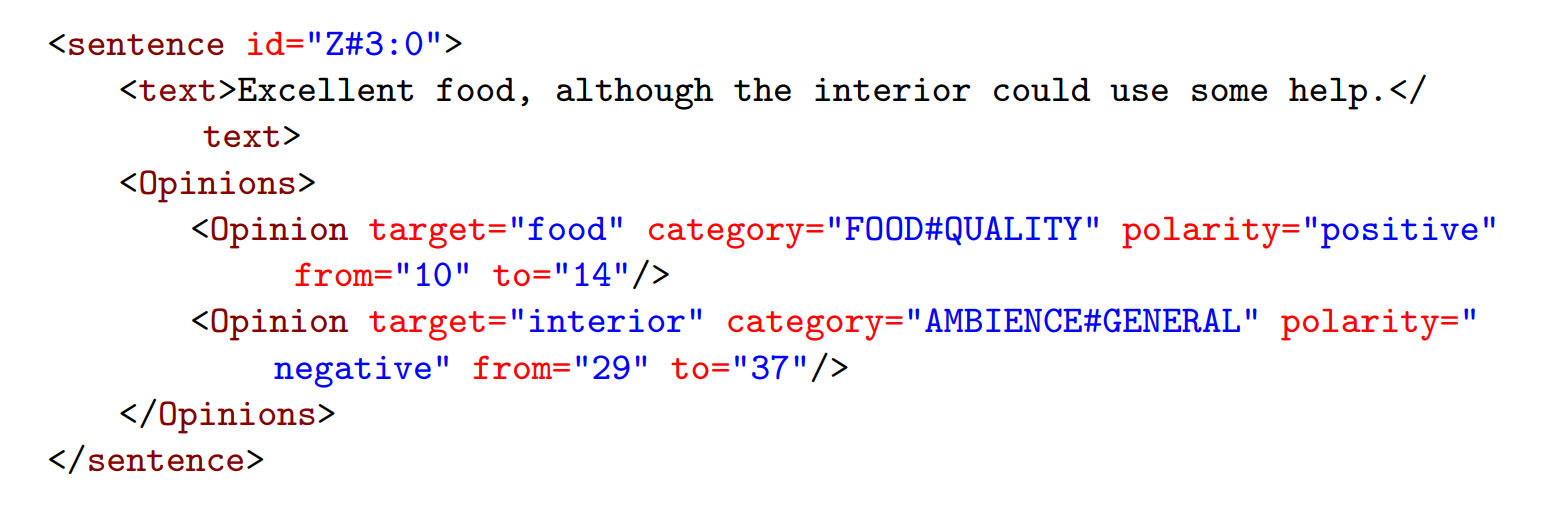
\includegraphics[width=0.9\textwidth]{example_semeval.PNG}
    \caption{A sentence from the SemEval 2016 dataset.}
    \label{fig:example_semeval}
\end{figure}

\section{Training dataset} \label{sec:training_data}
For our training dataset, we use the Yelp dataset challenge prepared by \textcite{Huang2020JASen} consisting of 17,027 unlabeled review sentences. The original dataset \parencite{Tang2016Yelp} contains many more data attributes. However, only the review text is extracted without any further modification. This dataset is chosen as it resides in the restaurant domain just like our evaluation data. Furthermore, this dataset is much larger compared to the SemEval dataset. While it does not include aspect-level information, it will not be needed due to the unsupervised nature of the model.

%%%%%%%%%%%%%%%%%%%%%%%%%%%%%%%%%%%%%%%%%%%%%%%%%%%%%%%%%%%%%%%%
\chapter{Methodology} \label{chap:methodology}

This chapter explains the models used in this research. First, \cref{sec:formulation} formulates the problem and introduces general notation to the task. Then, \cref{sec:CASC} explains the CASC model in detail. Next, \cref{sec:LCR-Rot} describes the neural model in detail and how it can be injected in CASC.

\section{Task Formulation} \label{sec:formulation} % A BIT SHORT BUT WHAT DO I ADD AGAIN?
We formulate the approach as a single-label multi-class classification problem, meaning that the output can only be one class from multiple classes. Let the input be a corpus $\mathcal{D} = [X_1, X_2, \dots, X_n]$ consisting of $n$ unlabeled review sentences from a domain. Given the set of aspect categories $A$ together with a small list of seed words $L_a$ for each aspect category $a \in A$, and sentiment polarities $S$ along with a small list of seed words $L_s$ for each sentiment polarity $s \in S$, the objective is to predict a pair of $(a, s)$ for a given unseen review sentence.

\section{Modified CASC} \label{sec:CASC}
This section describes the CASC model in detail. It consists of three different stages. In the first step, class vocabularies for aspect and sentiment categories are constructed through contextual embeddings using only seed words. Second, unlabeled data is turned into labeled data in a weakly-supervised manner using overlap scores with the vocabularies from the previous step. Third and last, a simple neural model with a linear layer is implemented to perform ACD and ASC.

\subsection{Class Vocabulary Construction}
With a small set of seed words $L_a$ corresponding to aspect $a \in A$, we find the set of sentences $X_a \subset \mathcal{D}$ which contain any of the seed words. Afterwards, sentence $X_i \in X_a$ is passed to a post-trained Domain Knowledge BERT Masked Language Model (DK-BERT MLM) to predict words for finding replacement candidates of all tokens in the sentence. DK-BERT MLM outputs replacement probability scores $P_i \in \mathbb{R}^{\lvert X_i \rvert \times \lvert V \rvert}$ with V being the vocabulary set used by DK-BERT. However, only replacement candidates of the tokens in the seed words are considered. Next, those replacement candidates are passed through a filter to get rid of stop words and punctuation. Then, the top $K$ words are selected as replacement candidates $R_i$ based on their probability scores computed by DK-BERT MLM. All replacement candidates $R_i$ for all $X_i \in X_a$ are collected and added to a frequency table corresponding to each $a \in A$. Subsequently, the top $M$ most frequent words for aspect category $a$ are selected to construct the aspect vocabulary set $V_a$. Last, words that appear inside multiple vocabularies are removed in both sets. A similar procedure is used to construct the sentiment vocabularies $V_s$ for all $s \in S$.

The intuition behind these steps is that words within a sentence can be replaced by words that carry a similar contextual meaning. DK-BERT MLM is trained to provide such replacement candidates such that the words outputted will resemble the meanings of the seed words closely. Furthermore, the vocabulary sets are disjoint sets to remove ambiguities across aspect and sentiment classes. The filter, which removes stop words and punctuation, further helps the procedure to minimize the overlap between vocabulary sets.

\begin{figure}[htbp]
  \centering
  \includesvg[width=0.5\textwidth]{CASC1.svg}
  \caption{}
  \label{fig:casc1}
\end{figure}

\subsection{Labeled Data Preparation} \label{sec:labeler}
Following the work by \textcite{Hu2004Rules}, the CASC model exploits the notion of aspects and opinion terms to be nouns and adjectives or adverbs, respectively. Therefore, nouns, adjectives, and adverbs are extracted using a POS tagger as \textit{potential-aspects} and \textit{potential-opinions}. % However, we propose a method to extract multiple aspect expressions per sentence instead of a single term.

First, we find the set of all sentences $X_q \subset \mathcal{D}$ which contains at least one \textit{potential-aspect} and one \textit{potential-opinion}. Then, sentence $X_j \in X_a$ gets passed through DK-BERT MLM to find replacement candidates with probability scores for each \textit{potential-aspect}. With these replacement candidates, the list $G_{aspect}$ is created by taking top K replacement words based on the probability scores. For sentence $X_j$, we find overlap score $S_a$ of each aspect $a \in A$ by counting the common words between its corresponding aspect vocabulary $V_a$ and the list $G_{aspect}$. Overlap scores for sentences $X_q$ with all aspect categories $A$ are stored in a score matrix $\mathcal{M} \in \mathbb{R}^{\lvert X_q \rvert \times \lvert A \rvert}$.

% \todo{Write about averaging vs maximum}

The vocabularies in the previous step were created with DK-BERT which is post-trained using a real-world domain-specific dataset. \textcite{Kumar2021CASC} argue that these datasets are often imbalanced. Some aspect categories appear much less or much more compared than others. This means that certain vocabularies contain a relatively larger number of semantically coherent words compared to other vocabularies. This difference in quality will affect the variance of the overlap scores per category. Therefore, the overlap scores per category are normalized:

\begin{equation}
    S'_{ja} = \frac{S_{ja} - \mu_{ja}}{\sigma_{ja}},
\end{equation}

\noindent where $S'_{ja}$ is the normalized overlap score of each aspect $a$ corresponding to sentence $X_j$, and $\mu_{ja}$ and $\sigma_{ja}$ are the mean and standard deviations of the overlap scores, respectively, and are computed as follows:

\begin{align}
    \mu_{ja}    & = \frac{1}{\lvert X_q \rvert} \sum_{j=1}^{\lvert X_q \rvert} \mathcal{M}_{ja}, \\
    \sigma_{ja} & = \frac{1}{\lvert X_q \rvert} \sum_{j=1}^{\lvert X_q \rvert} \left ( \mathcal{M}_{ja} - \mu_{ja} \right )^2.
\end{align}

The normalized score $S'_{ja}$ shows how many standard deviations the original score $S_{ja}$ away from the mean value is. For sentence $X_q$, aspect categories are assigned if the normalized score is above a pre-defined threshold $\lambda$. 
% \todo{assumption: one or multiple expression terms for aspect categories?} 
A similar procedure is applied for sentiment categories. With the previous steps completed, a labeled dataset $\mathcal{D}_\mathcal{L} \subset \mathcal{D}$ can be constructed which is a subset of the original corpus.

\begin{figure}[htbp]
  \centering
  \includesvg[width=0.5\textwidth]{CASC2.svg}
  \caption{}
  \label{fig:casc2}
\end{figure}

%%%% Extensions
Building on the original CASC model, the aspect term is extracted in this phase. During the aspect label assignment process, each aspect label $a$ gets an aspect term for each sentence $X$. Similar to the overlap scores, aspects are stored in a matrix. When the aspect label is decided, the corresponding aspect term is assigned to the sentence.

There are multiple ways of assigning aspect. The simplest method would be to assign the noun with the highest overlap score. Another approach could be to identify noun chunks \parencite{Honnibal2020Spacy} and select chunks with the highest averaged overlap scores. 
% \todo{I have not decided what would feasible given the time}

% https://stackoverflow.com/questions/44661200/spacy-to-extract-specific-noun-phrase

\subsection{Joint Neural Network for ACD and ASC} % Basically done
In the original CASC model, the authors used a simple yet effective neural model to classify aspects and sentiment. The authors make use of DK-BERT embeddings and extract the second-to-last hidden layer as embeddings for the tokens in the sentence. Sentences $X_l \in \mathcal{D_\mathcal{L}}$ are represented as $X_l = \left ( [CLS], w_1, \ldots, w_n, [SEP] \right )$, where $w_i$ represents a word in a sentence for $0 \leq i \leq n$. BERT considers the [CLS] and [SEP] as special tokens which denote the start and the end of a sequence, respectively. Therefore, the embeddings of the sequence is $H \in \mathbb{R}^{(n+2) \times d}$ for each token in $X_l$, where $d$ is the embedding size of the embedding layer, or in this case, the number of hidden layers in BERT. Afterwards, the global sentence representation $T \in \mathbb{R}^{1 \times d}$ is constructed by averaging embeddings from the non-special tokens: 
\begin{equation} 
    \frac{1}{n} \sum_{i=1}^{n}H_i. 
\end{equation}
Thus, the hidden representations of [CLS] and [SEP] are ignored. Last, the sentence representation $T$ is passed to two different linear layers for ACD and ASC: 
\begin{align}
    \hat{a} & = SoftMax(T \times W_a + b_a), \\
    \hat{s} & = SoftMax(T \times W_s + b_s),
\end{align}
where $W_a \in \mathbb{R}^{d \times \lvert A \rvert}$ and $W_s \in \mathbb{R}^{d \times \lvert S \rvert}$ are trainable weight matrices, and $b_a$ and $b_s$ are the trainable bias vectors. Last, $\hat{a}$ and  $\hat{s}$ denote the probabilities for the aspect category and sentiment polarity. 

\begin{figure}[htbp]
  \centering
  \includesvg[width=0.45\textwidth]{Simple Neural.svg}
  \caption{}
  \label{fig:simple_neural}
\end{figure}

However, the aspect term positions, extracted during the previous phase, are yet to be exploited in this neural model. Therefore, we suggest to inject the double task LCR-Rot-hop++ model instead of applying the neural model described above. 

\section{Double Task LCR-Rot-hop++} \label{sec:LCR-Rot}
This section describes the double task LCR-Rot-hop++ model \parencite{Trusca2020HAABSA++} in detail. This sophisticated model exploits positional information by using three Bidirectional Long Short Term Memory (BiLSTM) layers. Furthermore, two types of attention mechanisms are implemented in a iterative manner to exploit local and global contexts. This model replaces the third step of of the CASC model described in \cref{sec:CASC}. The LCR-Rot model was originally solely built for ASC. Therefore, a slight modification will be made to also handle ACD tasks.

Like before, DK-BERT is applied to generate embeddings. Unlike before, sentence $X_l$ is split into the left context, the target, and the right context of lengths $L$, $T$, and $R$, respectively. Moreover, the contexts are represented as $X_l^l = \left ( w_1^l, \ldots, w_L^l \right )$, $X_l^t = \left ( w_1^t, \ldots, w_T^t \right )$, and $X_l^r = \left ( w_1^r, \ldots, w_R^r \right )$, respectively, where $w_i^j$ represents the $i$th word in context $j$. To ensure that each context will have the same number of tokens, padding tokens $[PAD]$ are added if the sentence lacks tokens. Otherwise, contexts are truncated if there are too many tokens. Furthermore, separation tokens $[SEP]$ are added between the contexts to easily find the token length of each context. Note that the special tokens $[CLS]$ and $[SEP]$ are ignored after embedding. Therefore, the embeddings of a sentence are expressed as $H^l \in \mathbb{R}^{L \times d}$, $H^t \in \mathbb{R}^{T \times d}$, and $H^r \in \mathbb{R}^{R \times d}$. Following, each embedding part feeds separate BiLSTM layers which produce hidden states $B^l = \left( b_1^l, \dots, b_L^l \right)$, $B^t = \left( b_1^t, \dots, b_T^t \right)$, and $B^r = \left( b_1^r, \dots, b_R^r \right)$. Here, $b_i^j \in \mathbb{R}^{2d}$ represents the hidden state from the $i$th BiLSTM layer of context $j$.

Then, a three-step attention mechanism is iteratively applied over the three hidden states. The first and second mechanisms are rotary attention mechanisms which exploit local information, whereas the third is a hierarchical attention mechanism exploits global information. First, new left and right context representations are generated by using old target information. Second, two new target representations are generated by using the context representations produced in first step. Third, the phrase representations are updated by interacting the left and right contexts. The following paragraphs go in the mathematical detail of the procedures.

First, rotary attention mechanisms are applied. The new context representations are a weighted sum of the hidden states of each context: 

\begin{equation}
    r^c = B^{c\top} \times \alpha^c, \label{eq:rot_att}
\end{equation}

\noindent where $c$ denotes the left or right context $\{l, r\}$ consisting of $C$ words. Note that $C$ equals either $L$ or $R$ mentioned above. Furthermore, $B^c \in \mathbb{R}^{C \times 2d}$ corresponds to the hidden states for context $c$, and $\alpha \in \mathbb{R}^{C}$ denotes the attention weights assigned to each hidden state and is computed by the following function and applying the softmax function afterwards:

\begin{align}
    \alpha^c                         & = \text{softmax}\left( f \left( B^c, r^t\right) \right), \label{eq:alpha}\\
    f \left( B^c, r^t; c, t \right) & = \tanh{\left( B^{c\top} \times W^c \times r^t + b^c \times \mathbf{1} \right)}, \label{eq:tanh}
\end{align}

\noindent where $t$ denotes the left or right target $\{t_l, t_r\}$ consisting of $T$ words (distinction is explained in the next step). Note that this $T$ is the same one mentioned above. Furthermore, $r^t \in \mathbb{R}^{2d}$ corresponds to the target representation of target side $c$, and $\mathbf{1} \in \mathbb{R}^{C}$ denotes a vector of ones. Then, the trainable parameters are the weight matrix $W^c \in \mathbb{R}^{2d \times 2d}$ and the bias scalar $b^c \in \mathbb{R}$.

In the first iteration, there is no old target information to use. Therefore, the hidden states from the target phrase are averaged by using an average pooling layer resulting in target representation $r^t \in \mathbb{R}^{2d}$. In other iterations, target representations $r^t$, computed in step two (the next step), are used.

Second, another rotary attention mechanism is applied afterwards to generate the left and right target representations. Two target representations are generated to exploit context representations separately. Thus, the left target representation uses the left context and the right target the right context. The computations follow \cref{eq:rot_att,eq:alpha,eq:tanh} in a similar way. However, the $c$'s and $t$'s are swapped in this step, thus changing dimensions containing size $C$ to $T$, and vice versa.

Third, a hierarchical attention mechanism is applied to expoit global information. Intuitively, the mechanism decides whether the left or right context provides more relevant information about the target. The left and right contexts are scaled with each other. Furthermore, the left and right targets are scaled as well, but separately from the contexts. In short, each phrase representation is scaled by a scalar:

\begin{equation}
    \hat{r}^p = \alpha^{p\top} \times I_2 \times  r^p , \label{eq:hier_att}
\end{equation}

\noindent where $r^p \in \mathbb{R}^{2 \times 2d}$ denotes the vertically concatenated contexts $[r^l; r^r]$ or targets $[r^{t_l}; r^{t_r}]$ decided by $p$, and $I_n \in \mathbb{R}^{n \times n}$ denotes the identity matrix. Then, $\alpha^p \in \mathbb{R}^2$ denotes the attention weight vector assigned to each representation and is computed by applying the following function and softmax function:

\begin{align}
    \alpha^p                         & = \text{softmax}\left( f \left( r^p\right) \right), \label{eq:hier_alpha}\\
    f \left( r^p; p \right) & = \tanh{\left( r^{p} \times W^p + b^p \times \mathbf{1} \right)}, \label{eq:hier_tanh}
\end{align}

\noindent where the trainable parameters are the weight vector $W^p \in \mathbb{R}^{2d}$ and the bias scalar $b^p \in \mathbb{R}$. 

Last, all four representation vectors are horizontally concatenated and feed a dense layer with a softmax function and bias vector for the sentiment prediction. However, the original model does not classify the aspect category. Therefore, we extend the LCR-Rot-hop++ model. Modifying this neural model is inspired by the CASC model described above. Instead of passing the sequence representation through a single layer, two dense layers are instantiated for the ACD and ASC tasks. The ASC branch stays identical. The difference for the ACD task is that its layer has its own weight matrix and bias vector. \cref{fig:CASC+LCR} shows the visual representation of the neural model.

\begin{figure}[htbp]
  \centering
  \includesvg[width=0.9\textwidth]{CASC+LCR.svg}
  \caption{}
  \label{fig:CASC+LCR}
\end{figure}

\section{Experimental Setup} \label{sec:setup}
\subsection{Training Procedure} \label{sec:training}
Each model is trained in a similar fashion to \textcite{Kumar2021CASC}. The model minimizes a General Cross Entropy (GCE) function, which exploits both the Categorical Cross Entropy (CCE) and Mean Absolute Error (MAE). % cite zhang et al. Generalized cross entropy loss for training deep neural networks with noisy labels
CCE converges quickly but overfits to noise, while MAE is robust to noise but converges slowly. It has been shown that GCE performs better than CCE \parencite{Kumar2021CASC}. This makes intuitive sense as the dataset is semi-automatically labeled which introduces noise while annotating. In short, GCE de-emphasizes difficult samples compared to CCE but accentuate them more compared to MAE during training. Therefore, the aspect category classification loss $\mathcal{L}_a$ and sentiment polarity classification loss $\mathcal{L}_s$ are defined as follows:

\begin{align}
  \mathcal{L}_a & = \frac{1 - \left( \hat{a}_{y_a} \right)^q} {q}, \\
  \mathcal{L}_s & = \frac{1 - \left( \hat{s}_{y_s} \right)^q} {q},
\end{align}

\noindent where $\hat{a}_{y_a}$ and $\hat{s}_{y_s}$ denote the predicted probabilites against the true aspect and sentiment labels, and $q \in (0, 1)$ is a hyperparameter. The unregularized overall loss L of our model is the sum of both the losses $\mathcal{L}_a$ and $\mathcal{L}_s$:

\begin{equation}
    \mathcal{L} = \mathcal{L}_a + \mathcal{L}_s.
\end{equation}

Furthermore, $L_1$ and $L_2$ regularizations are applied to avoid overfitting. The regularization deems necessary as the neural model has become more sophisticated. It has more layers and more trainable parameters meaning that those parameters may cause the model to overfit easily. Therefore, the regularized loss is defined as follows:

\begin{equation}
    \mathcal{L} = \mathcal{L}_a + \mathcal{L}_s + \lambda_1 \|\Theta\|_1 + \lambda_2  \|\Theta\|^2_2,
\end{equation}

\noindent where $\lambda_1$ and $\lambda_2$ are the weights of the $L_1$ and $L_2$ regularization terms, respectively, and $\Theta$ is the parameter set which contains $\{W^c, W^t, W^p, b^c, b^t, b^p\}$ and the BiLSTM parameters.

For loss minimization, weight matrices described above are randomly initialized by a uniform distribution $U(-0.1, 0.1)$ and biases are set to zero. The rest of the parameters are set using the default settings provided by TensorFlow. The algorithm used to minimize the loss is Adam. % cite
Hyperparameters are tuned by using the Hyperband algorithm. % cite



%%%%%%%%%%%%%%%%%%%%%%%%%%%%%%%%%%%%%%%%%%%%%%%%%%%%%%%%%%%%%%%%
%%%%  The planning chapter will removed after the proposal  %%%%
%%%%%%%%%%%%%%%%%%%%%%%%%%%%%%%%%%%%%%%%%%%%%%%%%%%%%%%%%%%%%%%%

% \chapter{Planning} \label{chap:planning}
% The figure below shows my rough schedule for the thesis. If time allows, I will tinker with different ATE which is colored light orange. The finishing phase and resit phase are not colored as I do not know what to expect.

% \begin{figure}[htbp]
%     \centering
%     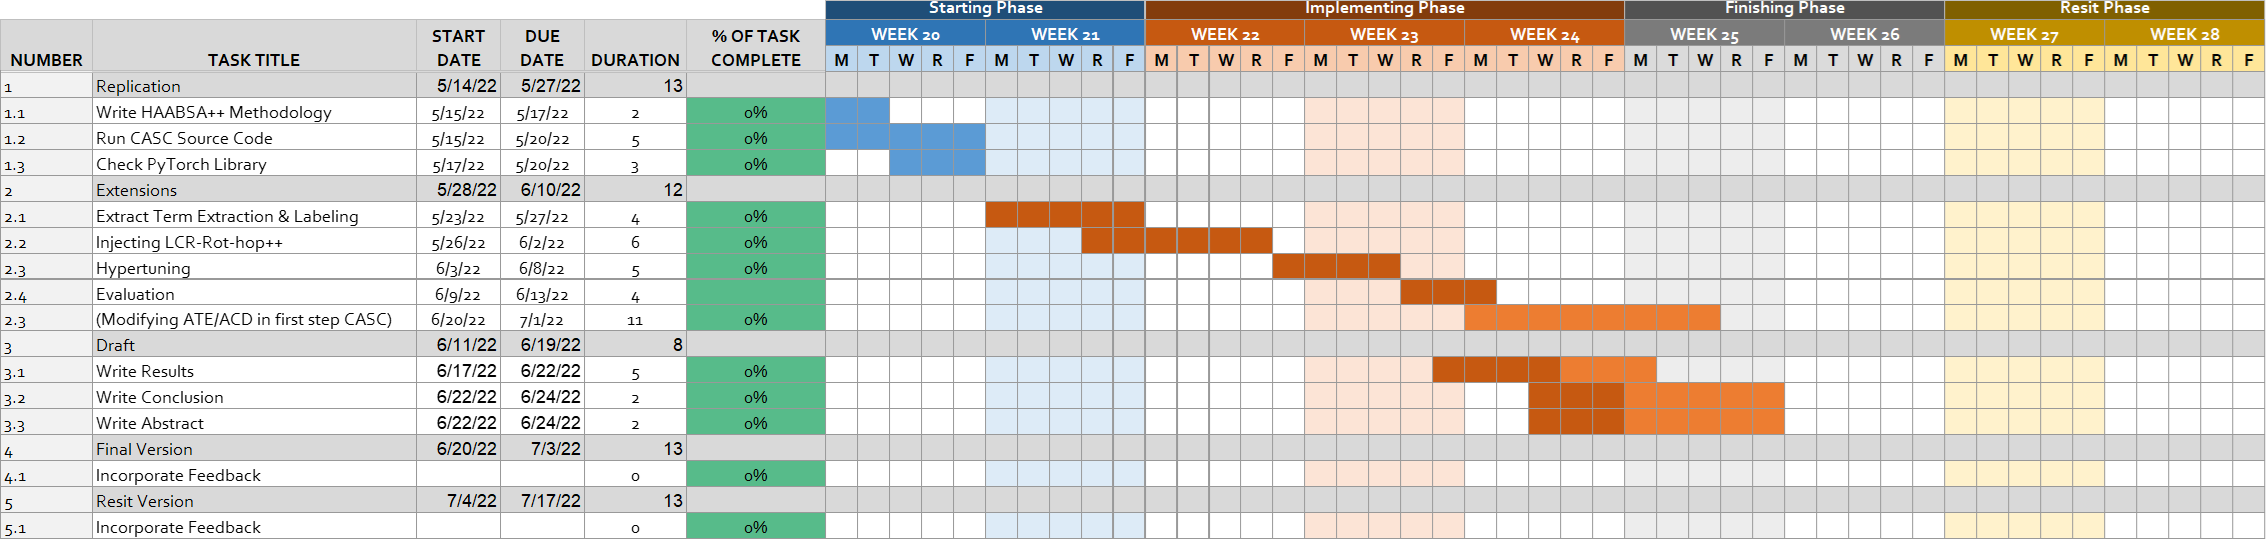
\includegraphics[width=1.5\textwidth, angle=90]{planning_gantt.png}
%     \caption{The rough schedule for my thesis}
%     \label{fig:planning}
% \end{figure}

%%%%%%%%%%%%%%%%%%%%%%%%%%%%%%%%%%%%%%%%%%%%%%%%%%%%%%%%%%%%%%%%
\chapter{Results} \label{chap:results}

\section{Performance Measures \& Baseline Models} \label{sec:baselines}
We evaluate the predictive performance of the models using out-of-sample accuracy and macro F1 scores. Both the aspect category classification and sentiment classification performance are evaluated. This paper mainly compares the novel model against versions of the CASC model. This is because the CASC model has shown to outperform previous models by quite a significant amount. Furthermore, at the time of writing, the CASC model is new and has seen no competition yet. The following models are compared:

\begin{itemize}
    \item CASC: The model framework presented by \textcite{Kumar2021CASC} using post-trained DK BERT-MLM and a small set of seed words for preparing labeled data. It then uses a simple neural network using labeled data for aspect and sentiment prediction.
    \item CASC+MAX: We use the score that corresponds to the word that has the maximum score amongst all other potential-aspects and potential-opinions in a sentence. Sentences are labeled according to the maximum score. For aspect categories, the CASC model uses averages the score over all potential-aspects per aspect category before taking the selecting the category with the highest score. 
    \item CASC+MAX+ATE: Additionally to the previous model, it extracts the aspect target expression. Similar to the LCR + CASC model, this model introduces a [SEP] token before and after the target expression. This way, we provide target location in the simplest form and can investigate how the simple neural model processes the information.
    \item LCR+CASC: Our full model framework building on the CASC + MAX + ATE model. We replace the simple linear neural model by the sophisticated LCR-Rot-hop++ neural model.
    \item LCR+CASC-DL: We omit the neural model altogether and use the same labeler described in \cref{sec:labeler}. We name this method LCR + CASC - DL, but is equivalent to CASC + MAX + ATE - DL.
    \item LCR+CASC-CON: We remove the left- and right-context-aware BiLSTM output in the last prediction layer. Thereby only using the concatenated target representations $\{r^t_l, r^t_r\}$.
    \item LCR+CASC+ASYNC: We create separate neural layers for each subtasks. Therefore, each task is solved in a asynchronous manner, whereas the LCR + CASC model shares most neural layers for both aspect and sentiment classification tasks.
    \item \ [MODEL] + SEP (GOLD): These types of models use the gold annotations provided by the SemEval datasets, instead of extracting the aspect target expressions using the labeler described in \cref{sec:labeler}. Note that the noisy training data is still generated using the maximum score together with the aspect target extraction. This way, we can isolate whether the score calculator or the neural model is driving factor of the performance results (of the testing data).
\end{itemize}


% \section{Ablation Models} \label{sec:ablation_models}
% The following set of models are variations of the \modelname model or the CASC model. They are also used in the ablation study in \cref{sec:ablation_study}. Therefore, the models presented are simplified models of the \modelname model that remove or replace complex parts into simpler ones. 


\section{Performance Results} \label{sec:performance}
In this section, we compare the different models described in \cref{sec:baselines} and compare them to each other. First, we use the test dataset without any gold annotations, whereas the next part of the analysis uses test data where sentences has been split into the correct contexts as the gold targets are given. Thus, the first part uses the labeler described in \cref{sec:labeler} to extract target expressions in a unsupervised manner.

We notice that CASC beats all other methods when it comes to aspect classification. Furthermore, it performs relatively well for sentiment classification. CASC beats LCR+CASC by a significant margin at aspect classification, whereas the performance comparison in sentiment classification is more ambiguous. CASC seems to struggle with the 2016 dataset at sentiment classification, while LCR+CASC has the worst performance for the 2015 data at sentiment classification compared to all neural models.

To understand the effectiveness of the different novel components, we perform an ablation study. With different components added to or deleted from methods, we can deduce the importance of each component and how they interact with others. We remove or add components as explained in \cref{sec:baselines} and we show their performances in \cref{tab:aspect-perf,tab:sentiment-perf} for aspect classification and for sentiment detection, respectively.

First, using the maximum score labeler instead of the average score labeler is detrimental to CASC's performance. There are two models which show the effect clearly. Omitting the neural model completely (LCR+CASC-DL) causes a large drop in performance. The performance drop is also larger than the CASC model without the neural network using the average labeler scorer presented in \textcite{Kumar2021CASC}. Furthermore, replacing the average labeler to the maximum score labeler in the CASC model causes the model to lose over 20 percentage points in the aspect classification task. However, it seems that the neural network is able to find the sentiment quite well by beating CASC for both datasets. This indicates that sentiment prediction is more robust than aspect class prediction. This might also be because the test data only includes sequences in which only one sentiment is being expressed.

Second, CASC with the aspect target extraction extension produces good results even though the maximum score labeler produces poor results. However, it performs worse than CASC in most situations since it only beat CASC in the 2016 dataset for the sentiment classification task. This result and the previous result indicate that the neural model is able to pick up some patterns if the location of the aspect is provided. Even though the target location information might not be perfect, the performance seems to be close to the original CASC's performance.

Third, the left and right context representations in the LCR+CASC model have a small but positive contribution for both aspect and sentiment classification. The LCR+CASC-CON sometimes even beats the full model in some of the cases. One possible reason could be that the two representations contain most relevant information of the contexts. The fluctuation of producing better results could be the consequence of poor target location information.

Fourth, the separation of neural layers has almost no difference in performance for the aspect classification task. However, the difference for the sentiment classification task in 2016 is a bit larger.

\begin{table}[htbp]
\centering
\caption{Performance of various methods on the aspect classification task}
\label{tab:aspect-perf}
% \resizebox{\textwidth}{!}{%
\begin{tabular}{@{\extracolsep{4pt}}lllll@{}}
\hline
Aspect         & 2015           &                & 2016           &                \\ \cline{2-3} \cline{4-5}
Model          & Acc            & Macro-F1       & Acc            & Macro-F1       \\ \hline
CASC           & \textbf{85.71} & \textbf{85.43} & \textbf{86.78} & \textbf{86.93} \\
CASC+MAX       & 64.52          & 63.51          & 65.70          & 64.46          \\
CASC+MAX+ATE   & 83.71          & 83.14          & 83.90          & 83.87          \\
LCR+CASC-DL    & 65.90          & 65.41          & 69.42          & 68.64          \\
LCR+CASC-CON   & 79.78          & 79.58          & 83.41          & 83.43          \\
LCR+CASC+ASYNC & 80.90	        & 80.43	         &82.93	          & 83.12          \\
LCR+CASC       & 80.90          & 80.44          & 82.44          & 82.52          \\ \hline
\end{tabular}%
% }
\end{table}

\begin{table}[htbp]
\centering
\caption{Performance of various methods on the sentiment classification task}
\label{tab:sentiment-perf}
% \resizebox{\textwidth}{!}{%
\begin{tabular}{@{\extracolsep{4pt}}lllll@{}}
\hline
Sentiment      & 2015           &                & 2016           &                \\ \cline{2-3} \cline{4-5}
Model          & Acc            & Macro-F1       & Acc            & Macro-F1       \\ \hline
CASC           & 90.32          & 90.20          & 87.19          & 82.92          \\
CASC+MAX       & \textbf{92.17} & \textbf{92.01} & 88.84          & 84.41          \\
CASC+MAX+ATE   & 89.89          & 89.84          & 89.76          & 86.56          \\
LCR+CASC-DL    & 68.66          & 68.37          & 57.44          & 55.29          \\
LCR+CASC-CON   & 88.76          & 88.65          & 93.17          & 90.61          \\
LCR+CASC+ASYNC & 89.89	        & 89.78	         & 91.22	      & 87.93          \\
LCR+CASC       & 88.20          & 88.07          & \textbf{94.15} & \textbf{91.84} \\ \hline
\end{tabular}%
% }
\end{table}

The next part of the analysis uses the gold annotations provided in the datasets. We ought to investigate these data to understand if persuing more complex models is worth studying. As shown by previous results, complex models do not necessarily produce better results. However, the results also show that the maximum score labeler produces poor results, this might indicate that the ATE part of the model has to be improved. By skipping the ATE task for the test data and using the already prepared target expressions, we investigate what the potential of sophisticated methods could be. Furthermore, sentences can now have multiple aspects. Therefore, the analysis is extended to investigate the performance on sentences with multiple aspects rather than single aspects. Note that the training data stays remains unchanged.

First, as suspected, the CASC model produces poor results with sentences including multiple aspects. The LCR+CASC model, on the other hand, does not struggle at all when it comes to multi-labeled data. It seems that more sophisticated models perform better at the aspect classification task in all situation. However, simple neural models perform similarly on sentiment classification. On a similar note, CASC performs quite well on the multi-labeled sentiment classification task. Both observations could be explained by how the data is constructed. Reviews are usually biased because everyone with internet acces can post a review. People want to recommend people to or deter people from a place. Therefore, one review most likely has only one sentiment. Furthermore, our data looks at sentences, making the likelihood to have a one sentiment much larger.

Second, CASC will produce much better results for sequences with multiple aspects if it could use target expression location information. Even with the simplest form of the information, providing a separation token before and after the target expression, its performance is on par with singly labeled sequences. Furthermore, similar to our earlier result, performance gains from single- to multi-label in the aspect classification task are greater than the gains in the sentiment classification task. Again, this is likely due to sequences including multiple aspects express the same sentiment over multiple aspects.

% This indicates that labeling by averaging scores across all potential-aspects or potential-nouns is better than labeling the sequence by the maximum score. However, this reasoning is a bit ambiguous as it is not backed up by the previous result. In the previous result, labeling is also done on the maximum score, but performance is always better for aspect classification and quite close for sentiment classification.

Third, unlike before, removing the left and right context in the last dense layer hurts the model's performance. The difference with before indicates that the left and right contexts only contain useful information when the target expression is correctly given. In particular, the loss in performance is less for aspect classification than for the sentiment classification. Also, the multi-labeled performance deteriorates more than singly-labeled data in aspect classification. Logically, the aspect classification task depends much less on the context directly. It could depend more when multiple aspects are present. The target expression should provide enough information already if the target expression is indeed representative for the corresponding category. Meanwhile, sentiment depends more on context even though context information has been included through the attention layers. 

Fourth, unlike before, having separate neural layers per task shows the benefits of solving them in a multi-task manner. The LCR+CASC+ASYNC model performs the best in all but one situation for the aspect classification task. While it got beaten the LCR+CASC model in every situation for the sentiment classification task. This indicates that the neural layers can share relevant information across tasks. However, it seems that some information has been lost on the aspect classification task.

\begin{table}[htbp]
\centering
\caption{Performance of various methods on the aspect classification task on gold annotated data}
\label{tab:aspect-perf-gold}
\resizebox{\textwidth}{!}{%
\begin{tabular}{@{\extracolsep{4pt}}lllllllll@{}}
\hline
Aspect                   & \multicolumn{4}{l}{Single}                                        & \multicolumn{4}{l}{Multi}                                         \\ \cline{2-5} \cline{6-9}
                         & 2015           &                & 2016           &                & 2015           &                & 2016           &                \\ \cline{2-3} \cline{4-5}   \cline{6-7} \cline{8-9}
Model                    & Acc            & Macro-F1       & Acc            & Macro-F1       & Acc            & Macro-F1       & Acc            & Macro-F1       \\ \hline
CASC+SEP(GOLD)           & 86.18          & 86.18          & 86.36          & 85.96          & 75.00          & 73.93          & 79.06          & 77.00          \\
CASC+MAX+ATE+SEP(GOLD)   & 84.33          & 83.73          & 89.67          & 88.90          & 85.56          & 85.03          & 85.56          & 84.86          \\
LCR+CASC-CON+SEP(GOLD)   & 90.78          & 91.27          & 94.21          & 94.80          & 92.03          & 91.80          & 93.14          & 92.97          \\ 
LCR+CASC+ASYNC+SEP(GOLD) & \textbf{94.47} & \textbf{94.71} & \textbf{95.87} & \textbf{95.17} & \textbf{94.83} & \textbf{94.52} & \textbf{94.77}	& 94.05          \\ 
LCR+CASC+SEP(GOLD)       & 92.63          & 93.28          & 94.63          & 94.96          & 93.53          & 93.36          & 94.22          & \textbf{94.10} \\ \hline
\end{tabular}%
}
\end{table}

\begin{table}[htbp]
\centering
\caption{Performance of various methods on the sentiment classification task on gold annotated data}
\label{tab:sentiment-perf-gold}
\resizebox{\textwidth}{!}{%
\begin{tabular}{@{\extracolsep{4pt}}lllllllll@{}}
\hline
Sentiment                & \multicolumn{4}{l}{Single}                                        & \multicolumn{4}{l}{Multi}                                         \\ \cline{2-5} \cline{6-9}
                         & 2015           &                & 2016           &                & 2015           &                & 2016           &                \\ \hline
Model                    & Acc            & Macro-F1       & Acc            & Macro-F1       & Acc            & Macro-F1       & Acc            & Macro-F1       \\
CASC+SEP(GOLD)           & \textbf{92.63} & \textbf{92.53} & 85.95          & 81.37          & 87.28          & \textbf{86.36} & 88.81          & 83.61          \\
CASC+MAX+ATE+SEP(GOLD)   & 89.40          & 88.99          & 88.43          & 83.31          & 87.50          & 86.13          & 90.07          & 84.24          \\
LCR+CASC-CON+SEP(GOLD)   & 86.64          & 86.17          & 91.74          & 87.58          & 84.70          & 83.14          & 92.06          & 87.44          \\ 
LCR+CASC+ASYNC+SEP(GOLD) & 89.40	      & 89.07	       & 91.32	        & 87.40	         & 85.99	      & 84.61	       & 91.88	        & 87.20          \\ 
LCR+CASC+SEP(GOLD)       & 89.86          & 89.36          & \textbf{93.80} & \textbf{90.33} & \textbf{87.93} & 86.35          & \textbf{92.96} & \textbf{88.33} \\ \hline
\end{tabular}%
}
\end{table}


%%%%%%%%%%%%%%%%%%%%%%%%%%%%%%%%%%%%%%%%%%%%%%%%%%%%%%%%%%%%%%%%
\chapter{Concluding Remarks} \label{chap:remarks}
\section{Conclusion} \label{sec:conclusion}
ABSA mainly aims to classify aspects and sentiment for every aspect in a sentence. Supervised ABSA models have been studied thoroughly but are constrained by the limited availability of training data. Unsupervised and weakly supervised methods have been constructed to overcome this limitation. This way, no labor is required to create labeled datasets, resulting in businesses of all sizes being able to implement these models.

In this study, we overcome this limitation by combining the state-of-the-art weakly-supervised CASC \parencite{Kumar2021CASC} and supervised LCR-Rot-hop++ \parencite{Trusca2020HAABSA++} models to classify aspect categories and sentiment polarity. The models were adapted and modified to work with each other. First, a new scoring method had to be constructed to extract the aspect target expression. Second, the sophisticated LCR-Rot-hop++ has been altered to also solve the ACD task.

The results show that the LCR+CASC model does not perform as well as the CASC model. However, it does see potential. Furthermore, it seems that the LCR+CASC model is able to detect what aspect category a target has. The weakness of the model lies in the ATE part of the model. Labeling and extracting a word with the highest aspect score, rather than labeling the sentence based on the average score, produces poor results. However, the LCR+CASC model does perform quite well if one does have aspect target expression information solely for the testing data. In this case, LCR+CASC beats CASC by a fair amount when it comes to multi-labeled sentences. Moreover, the components of the neural model seem to have an overall positive effect on the performance. Its effect gets better when the correct target expressions are given in the testing data. 

\section{Limitations \& Future Research} \label{sec:limitation}
Although CASC has seen great results on a different domain than restaurants, the LCR+CASC's performance is not yet known. Not much research has been done on the laptop domain of the SemEval datasets as they usually do not provide any aspect target expressions. As the LCR+CASC model is capable of ATE, it can be tested on that domain. 

Furthermore, results show that the ATE part of in the labeled data preparation step produces poor results. Rather than extracting words that have the highest score in a sentence, one could research the extraction of noun phrases or more advanced scoring methods besides taking averages or maxima.

Last, this paper focused on injecting the LCR-Rot-hop++ model into CASC. The limitation of this model is that this model needs the target location to separate the left and right contexts. Other neural models such as graph based neural networks could be researched and do not need any modification in the score calculator to do ATE.

% \cite{Devlin2019BERT}
% \cite{Devlin2019BERTold}

% PLEASE LET ME KNOW WHICH OF THESE VERSIONS OF THE REFERENCES YOU PREFER. THERE ARE SOME SUBTLE DIFFERENCES WHICH I DO NOT KNOW WHICH IS BETTER.

\backmatter
\printbibliography
% \bibliographystyle{plain}
% \bibliography{Latex/refs.bib}

\appendix


\end{document}
